\chapter{Terrain Fingerprints}
\label{chapter:FingerprintingATerrain}




% FOOTNOTE THE ATTRIBUTIONS
\let\thefootnote\relax\footnote{Portions of this chapter previously appeared as: FIX \bibentry{stuetzle-TerrainDistances} }







% Chapter \ref{chapter:DrillOperator} presented the drill operator, a mathematical description of a terrain surface. Section \ref{section:TerrainDistances} presented a series of metrics used to measure the distance between two terrain datasets based solely on the shape of their extracted channel networks and the spatial positions of their elevation points. 
The idea that the underlying mathematics of a terrain surface can be used as an accurate representation of terrain will be taken one step further in this chapter by introducing a method for representing the terrain as a series of statistical descriptors, and using these descriptors to define another distance metric for measuring terrain dissimilarity.

This chapter presents the idea of the \emph{fingerprint} of a terrain $T$. A terrain's fingerprint is a set of characteristics 
% displayed by the terrain that are
 drawn from the hydrographic channel network that can be extracted from the terrain as described in Section \ref{section:ChannelNetworkExtraction}. 
% Once the terrain's channel network is identified, a series of statistical and geometric characteristics are extracted, making up the terrain's fingerprint. 
These characteristics describe a variety of aspects of the terrain including 
% channel shape, 
drainage density, flow pattern, and individual pixel importance.


% A fingerprint provides a 
% % mostly 
% unique 
% description of a terrain surface. One important application is the determination of a measure of dissimilarity between two terrains by assigning a quantity to the distance between their fingerprints. The typical methods for measuring terrain distance, as described in Section \ref{section:DescriptionOfMetrics}, fail to capture the local differences in terrain hydrography. These differences would provide a more localized error metric.
% Quantitative and qualitative comparison of this error makes possible deeper analysis of channel network evolution, as well as leads directly to more useful methods for choosing the flow threshold values used during channel network extraction, as discussed in Section \ref{section:ChoosingAFlowThreshold}.
% 
Fingerprints also provide insight into the behavior of water on the terrain, because they are determined by the terrain's channel network. Many applications rely on determining water flow on a surface, including flood planning and dam siting. 

\section{Pixel Identification}
\label{section:PixelIdentification}

Firstly, a method for identifying and categorizing the pixels in the extracted channel network, $N_{\tau}$, is necessary. For this purpose, each pixel $\textbf{p}_{i} \in N_{\tau}$ 
% belonging to the extracted channel network after thresholding the flow
%  with positive flow remaining 
in assigned a designation. A pixel can be designated with one of five categorizations based on the flow direction of it and any of its eight neighbors that also reside in the extracted channel network. The term ``neighbor'' as used in this designation is restricted to those pixels within the channel network:
%  (the term ``non-zero neighbor'' refers to neighbors in the channel network): 

\begin{itemize}
  \item Channel Start (S): All neighbors carry flow {\em away} from this pixel.
  \item Channel End (E): All neighbors carry flow {\em into} this pixel. %  At least one neighbor must be non-zero.
  \item Channel Junction (J): Flows to exactly one neighbor, while more than one neighbor contributes to this pixel's flow.
  \item Channel (C): Exactly one neighbor contributes to the pixel's flow, and this pixel contributes to exactly one neighbor.
%   \item Island (I): All neighboring pixels have flow lower than the threshold.
\end{itemize}

\noindent 
% Note that an effective flow threshold should provide a network with few, if any, I pixels, and only when using a flow accumulation algorithm that does not guarantee flow off the edge of the terrain. 
It is 
% also 
important to note that, when using a flow accumulation algorithm in which a pixel's entire flow is applied to a single neighbor (as opposed to using a fractional flow method), channels can not split. An example of a channel network with designated start, end, and junction points is found in figure \ref{figure:channelPoints}.

\begin{figure*}[t]
\centering
\begin{minipage}[b]{0.9\linewidth}
\begin{center}
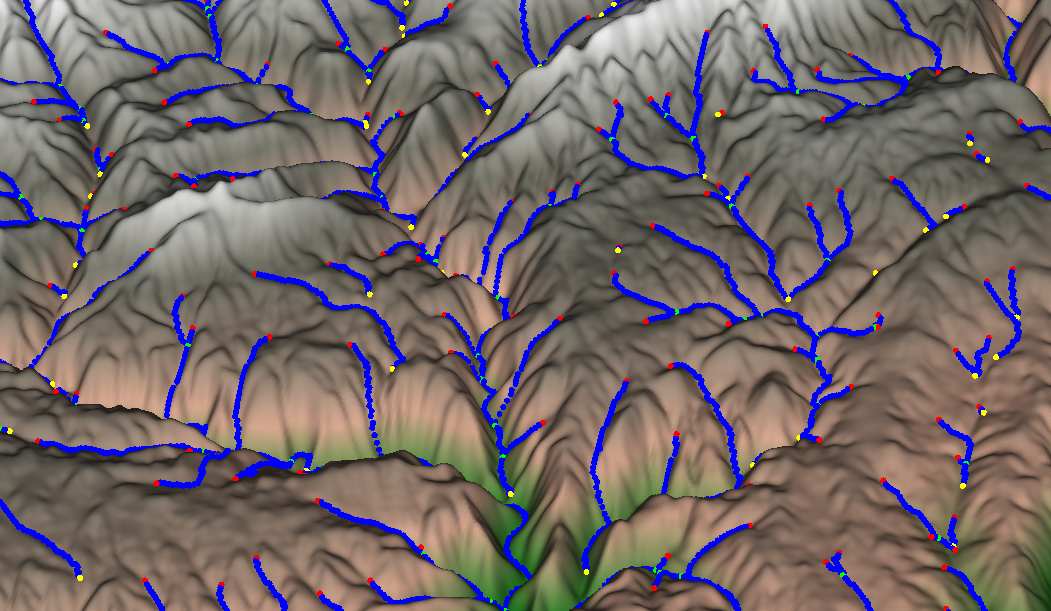
\includegraphics[width=\linewidth]{images/RiverGraph2_crop.png}
\end{center}
\end{minipage}
\caption[Channel pixel assignment visualization]{\label{figure:channelPoints}The pixels that make up the channel network are labeled based on incoming and outgoing flow, starting from each channel end. S pixels are red, J pixels are green, and E pixels are yellow.}
\end{figure*}

A more formal definition of a channel \emph{segment} than the one presented in Chapter \ref{chapter:DrillOperator} is a set of pixels connecting an S to an E, an S to a J, a J to a J, or a J to an E. Segments will consist of exactly two S, E, or J pixels and a series of 0 or more 8-connected contiguous C pixels. A channel \emph{network} is defined as a series of connected segments. Each network can contain any number of S pixels but exactly one E pixel.

To each network within a terrain we assign an i.d. $i$, so a network in $T$ is $N^{i}_{\tau}$. An \emph{address} is assigned to each pixel \textbf{p} in $N^i_{\tau}$, designating in which $N^i_{\tau}$ it is found. The process of assigning addresses to pixels is a recursive tree traversal algorithm that begins at an E pixel and adds another level to the address whenever a J pixel is encountered, ending at an S pixel. An illustration of this addressing scheme is found in Figure \ref{figure:addressingScheme}, and the procedure can be found in Algorithm \ref{algorithm:addressingScheme}.

\begin{figure*}[t]
\centering
\begin{minipage}[b]{0.9\linewidth}
\begin{center}
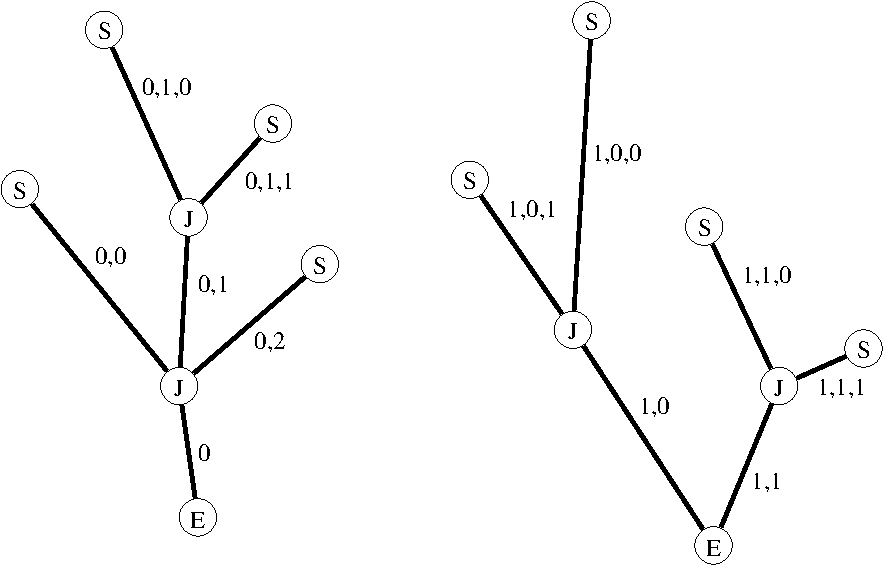
\includegraphics[width=\linewidth]{images/network_diagram.pdf}
\end{center}
\end{minipage}
\caption[Pixel addressing visualization]{\label{figure:addressingScheme}The segments and nodes that compose each channel network on the terrain are consistently labeled, starting from each channel end. This graphic shows two examples of the labeling and addressing scheme.}
\end{figure*}

\begin{algorithm}[t]
assignPixelAddress( pixel \textbf{p}, address )
\begin{algorithmic}
  \STATE $newChannels \gets 0$
  \STATE $Pnbrs = getPNeighbors( \textbf{p} )$ 
  \IF{ $Pnbrs > 1$ }
    \STATE $address.pushOntoBack( newChannels )$
    \STATE $newChannels \gets newChannels + 1$
  \ENDIF
  \FOR{ $i \in Pnbrs$ }
    \STATE $assignPixelAddress( i, address )$
    \IF{$ Pnbrs > 1$ }
      \STATE $address.popOffBack$
      \IF{$i + 1 < Pnbrs$}
	\STATE $address.pushOntoBack( newChannels )$
	\STATE $newChannels \gets newChannels + 1$	
      \ENDIF
    \ENDIF
  \ENDFOR
\end{algorithmic}
\caption[Pixel addressing algorithm]{\label{algorithm:addressingScheme}The method used to determine the address of each pixel in the channel network. The function $assignPixelAddress(\textbf{p}, address)$ is recursively called for each pixel in a depth first fashion, assigning the current address (a string of integers) to the current pixel, and then adjusting the back value of the address string for each additional neighbor of the pixel. Note that $getPNeighbors$ is a subroutine that returns only neighboring pixels in the channel network.}
\end{algorithm}

Once the pixels of the channel network have been identified, and their addresses have been assigned, the fingerprint may be calculated.



\section{Fingerprint Characteristics}
\label{section:FingerprintCharacteristics}

% There are two distinct types of fingerprint characteristics. The first is those that require a ``baseline'' terrain, $T_{0}$, to use as time 0 for a series of temporally evolving terrains. These characteristics are computed using erosion depth at each pixel, which can only be accurately obtained by comparing to a matching baseline, pre-eroded terrain. An example of a dataset that matches this description are those that are generated by the erosion computer simulation presenting in section \ref{section:ErosionSimulation}. The second type of characteristic is one which can be computed on any individual terrain. These data are generally easier to find, and are represented in this work by those in figure \ref{figure:SixDatasets}.

The three characteristics that comprise terrain fingerprints are
% channel width, channel depth, 
meander, pixel load, and junction balance. This section describes these characteristics in detail. Each characteristic is represented by an $X \times Y$ sparse matrix of values. All pixels not part of the extracted channel network contain values of 0. 
% 
It is critical to remember that each of the fingerprint characteristics discussed in this section are sensitive to small changes in the flow threshold values used to obtain the channel network. For this reason, the threshold for all channel networks used in this section is constant, a flow accumulation value of 160,
as seen in Figure \ref{figure:ChannelNetwork_GlobalThreshold}.

% \subsection{Channel Depth and Width}
% \label{section:ChannelDepthAndWidth}
% 
% The two terrain characteristics that require a baseline terrain for calculation are channel depth and channel width. These provide for a pixel-by-pixel cross section of the channels formed through the evolution of the terrain under erosion conditions. Channel depth is the simpler of the two. To compute, a difference field is calculated, which is simply the difference in elevation between $D_{0}$ and time step in question, $T_{t}$. Figure \ref{figure:ThreeTimeStepsWithDepthsAndWidths} shows a series of three time steps, at 1 minute, 5 minutes, and 9 minutes of an erosion simulation, as well as the corresponding depth fields.
% 
% % Figure of three time steps and their erosion depths
% \begin{figure*}[t]
% \centering
% \begin{minipage}{0.9\linewidth}
% \begin{tabular}{@{}r@{}|@{}c@{}|@{}c@{}|@{}c@{}|}
% Time~ & Terrain & Channel Depth & Channel Width \\
% \hline
% \begin{sideways}
% \begin{large}~~~~~1:00~~~~~\end{large}
% \end{sideways}
% ~
% &
%   \begin{minipage}[b]{0.32\linewidth}
%   \begin{center}
%   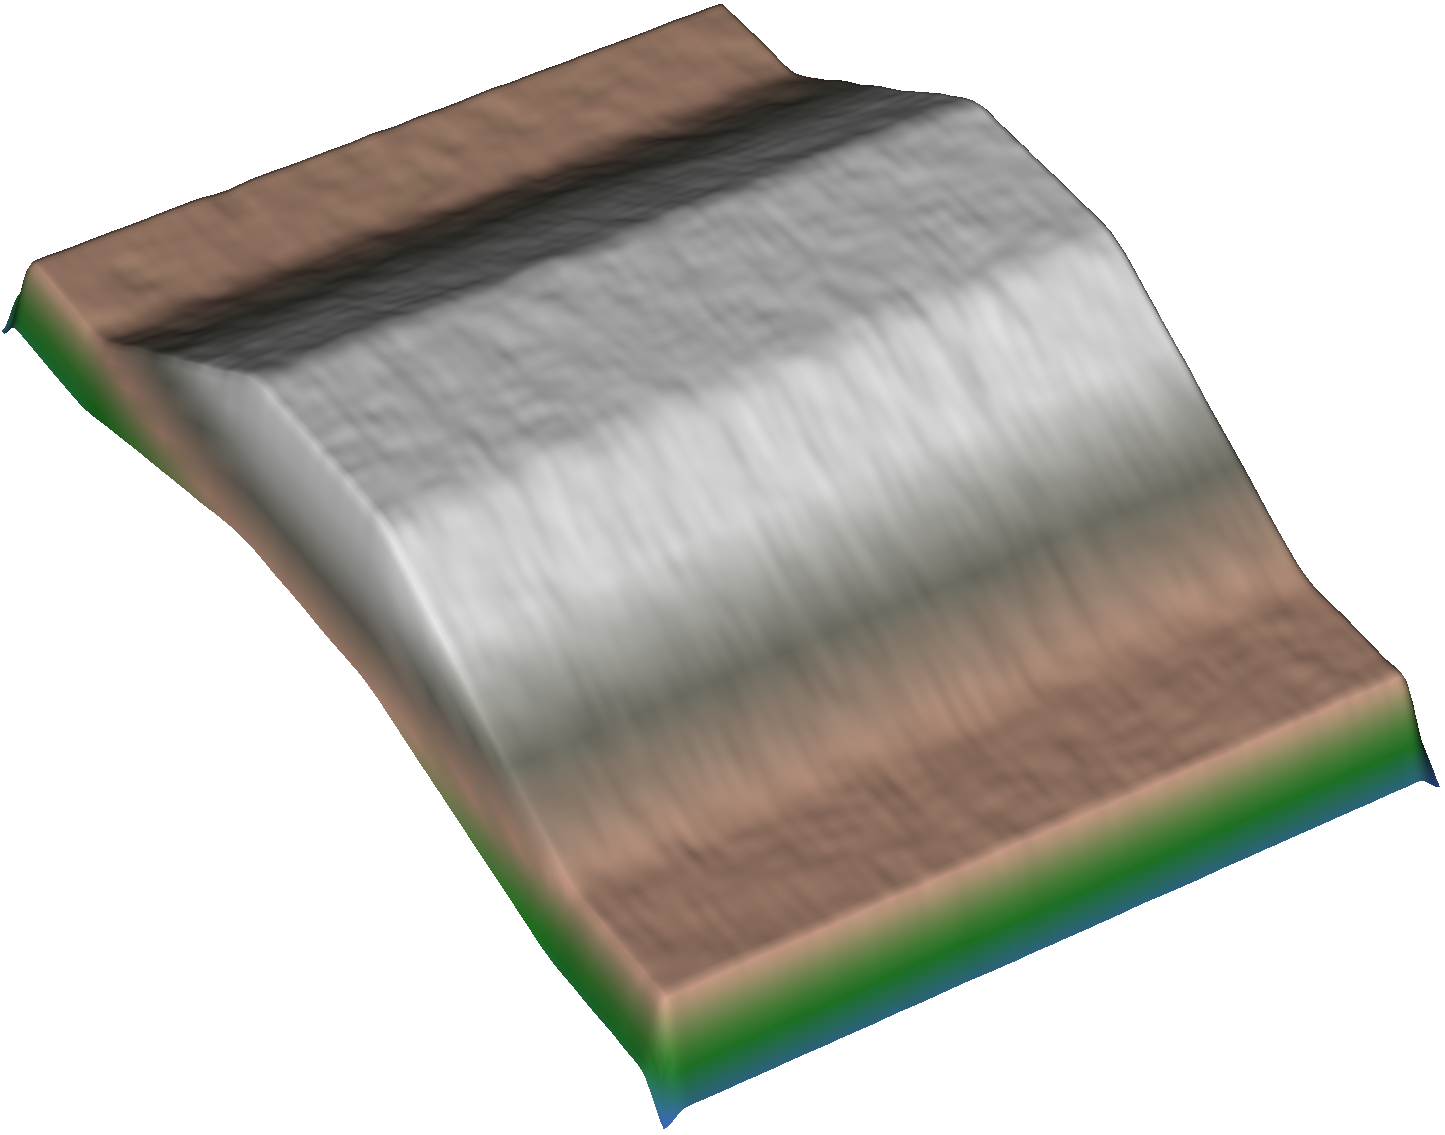
\includegraphics[height=0.13\textheight]{images/ErodedTerrain_TimeStep1.png} \\
%   \end{center}
%   \end{minipage}
% &
%   \begin{minipage}[b]{0.32\linewidth}
%   \begin{center}
%   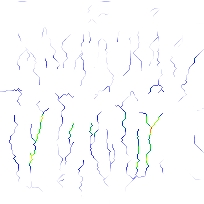
\includegraphics[height=0.13\textheight]{images/StatisticsTerrain1_ChannelDepth.jpg} \\
%   \end{center}
%   \end{minipage}
% &
%    \begin{minipage}[b]{0.32\linewidth}
%   \begin{center}
%   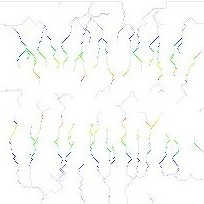
\includegraphics[height=0.13\textheight]{images/StatisticsTerrain1_ChannelWidth.jpg} \\
%   \end{center}
%   \end{minipage}
% \\ \hline
%   %
% \begin{sideways}
% \begin{large}~~~~~5:00~~~~~\end{large}
% \end{sideways}
% ~
% &
%   \begin{minipage}[b]{0.32\linewidth}
%   \begin{center}
%   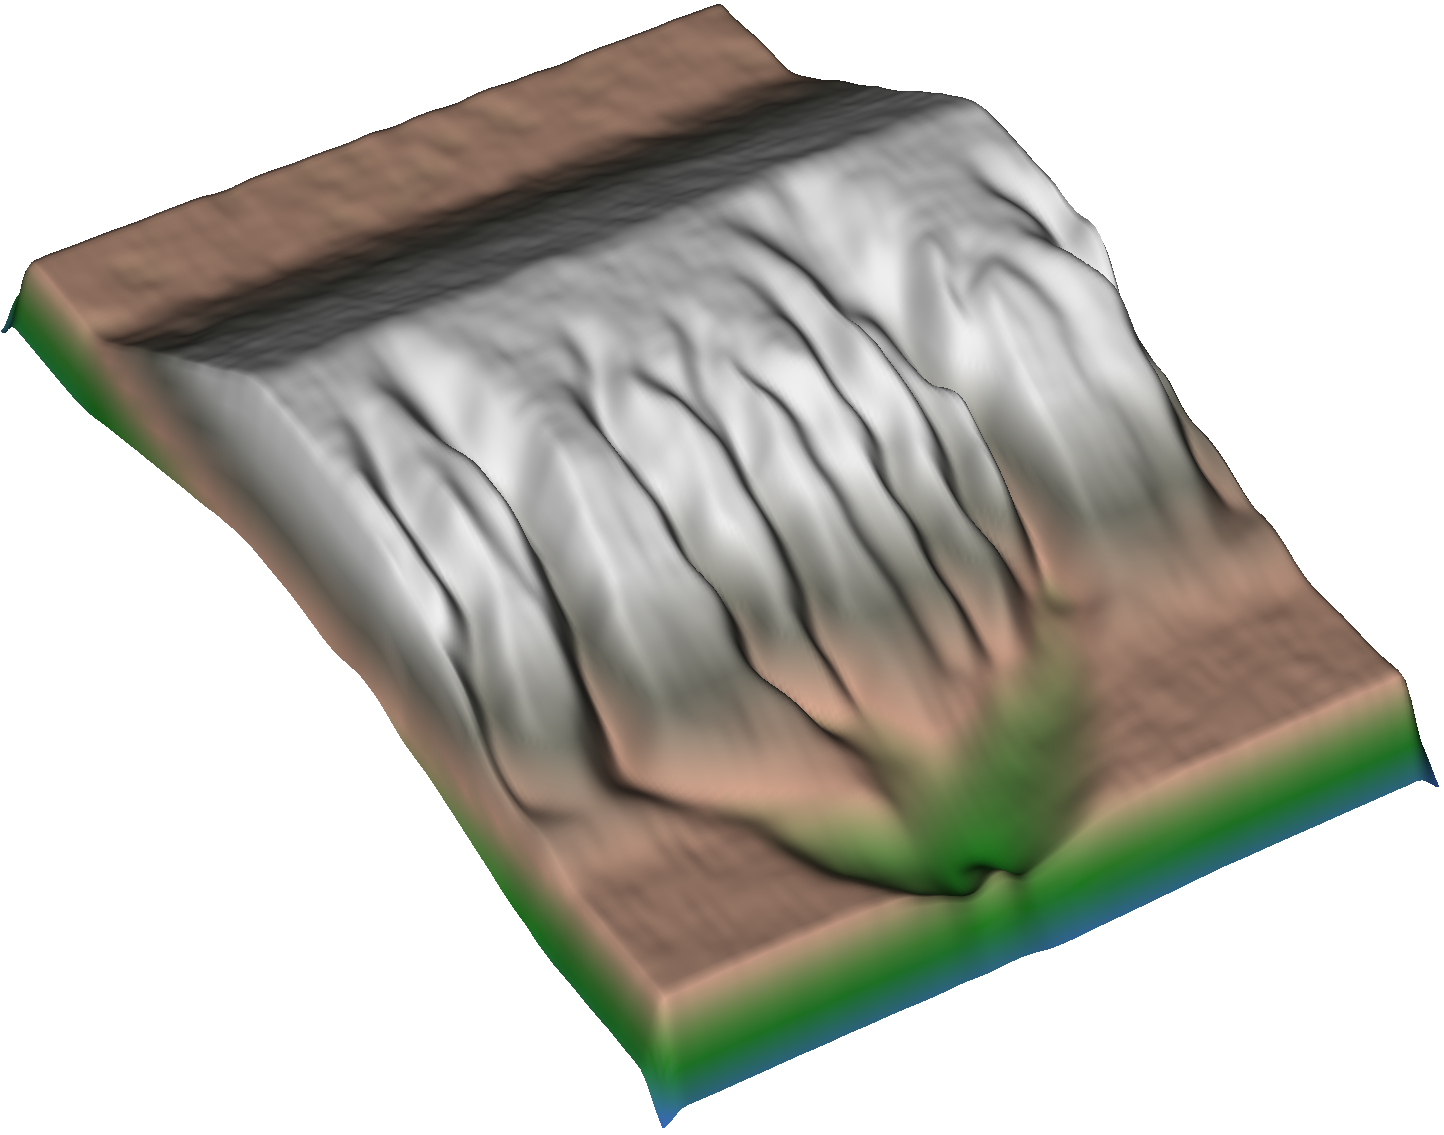
\includegraphics[height=0.13\textheight]{images/ErodedTerrain_TimeStep5.png} \\
%   \end{center}
%   \end{minipage}
% &
%   \begin{minipage}[b]{0.32\linewidth}
%   \begin{center}
%   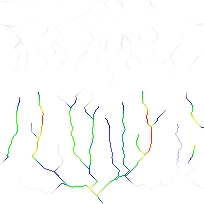
\includegraphics[height=0.13\textheight]{images/StatisticsTerrain5_ChannelDepth.jpg} \\
%   \end{center}
%   \end{minipage}
% &
%    \begin{minipage}[b]{0.32\linewidth}
%   \begin{center}
%   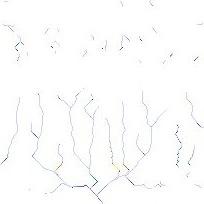
\includegraphics[height=0.13\textheight]{images/StatisticsTerrain5_ChannelWidth.jpg} \\
%   \end{center}
%   \end{minipage}
% \\ \hline
% \begin{sideways}
% \begin{large}~~~~~9:00~~~~~\end{large}
% \end{sideways}
% ~
% &
%   %
%   \begin{minipage}[b]{0.32\linewidth}
%   \begin{center}
%   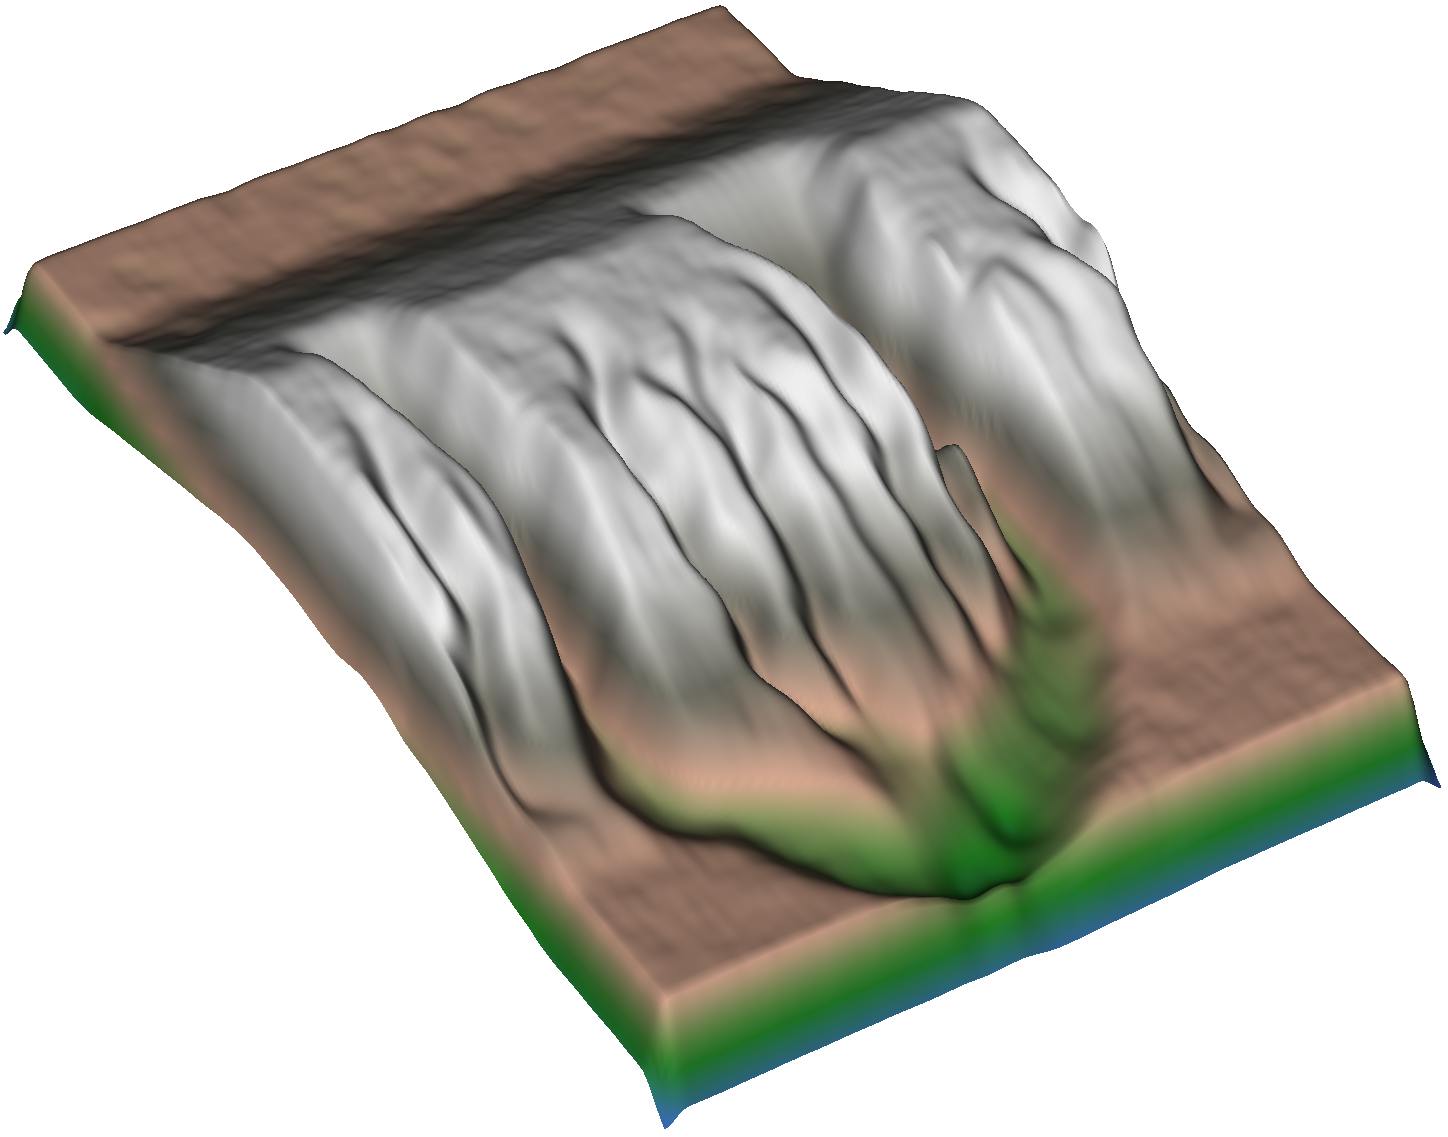
\includegraphics[height=0.13\textheight]{images/ErodedTerrain_TimeStep9.png} \\
%   \end{center}
%   \end{minipage}
% &
%   \begin{minipage}[b]{0.32\linewidth}
%   \begin{center}
%   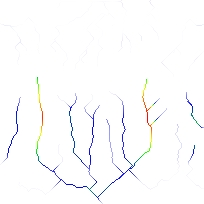
\includegraphics[height=0.13\textheight]{images/StatisticsTerrain9_ChannelDepth.jpg} \\
%   \end{center}
%   \end{minipage}
% &
%    \begin{minipage}[b]{0.32\linewidth}
%   \begin{center}
%   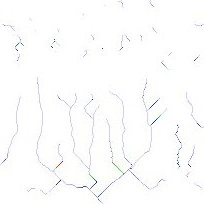
\includegraphics[height=0.13\textheight]{images/StatisticsTerrain9_ChannelWidth.jpg} \\
%   \end{center}
%   \end{minipage}
% \\ \hline
% \end{tabular}
% \end{minipage}
% %
% \caption[Channel depth and width visualization]{\label{figure:ThreeTimeStepsWithDepthsAndWidths}Three separate time steps of an erosion simulation. The geometry is a levee with a 5:1 slope, as seen in the left column. The center column displays a visualization of the depth at each pixel on the terrain, ranging from blue (little erosion depth) to red (significant erosion depth). The right column displays a visualization of the channel width field, ranging from blue (small width) to red (wide channels).}
% \end{figure*}
% 
% % Early in the simulation (time step 1:00) the erosion depth is scattered across the entire terrain, but as time passes it becomes much more localized to the channels that formed along the levee's downslope. Observe that very clear and well defined channel form as time passes. By the end of the simulation, it is possible to determine not only the boundaries of the channels, but also the deepest pixels, as well as some geometric properties. For instance, at the 9:00 mark, there are two major channels that have formed, one to the right and one to the left. However, the right channel flows around an uneroded plateau area, the dark blue patch just below the dark red area. This indicates a split in the flow of water.
% 
% Channel width is calculated for every pixel in the terrain, resulting in a channel width field in which every pixel is assigned a width value. Those pixels not in the channel network are assigned a value of 0. Width is calculated for a pixel \textbf{p} by determining the direction of flow from \textbf{p}, and walking along the terrain in each perpendicular (2D) direction until reaching either a pixel which has experienced no erosion, or until the walk is no longer uphill. In essence, this measures the distance one has to walk along the terrain until he is no longer walking uphill an eroded channel. It is important to note that the algorithm relies on the assumption that the channel pixels are the deepest pixels in the channel (because otherwise walking uphill would make no sense). This is an accurate assumption because, if it was not the case that the channel pixels were the lowest in a channel, then there would be pixels that the channel pixels would provide flow for, and thus there would be pixels with greater flow values. The procedure for calculation is described in Algorithm \ref{algorithm:ChannelWidth}.
% 
% \begin{algorithm}[t]
% \begin{algorithmic}
%   \FOR{$\textbf{p} = 0 \to numPixels$}
%     \STATE $dir \gets getDirectionsPerpToFlow( \textbf{p} )$
%     \STATE $newPix \gets \textbf{p}$
%     \STATE $lastPix \gets \textbf{p}$
%     \STATE $distance \gets 0$
%     \WHILE{$diffField[ newPix ] > 0 ~~\&\&~~ D[ newPix ] > D[ lastPix ]$}
%       \STATE $lastPix \gets newPix$
%       \STATE $newPix \gets getNextPix( dir, newPix )$
%     \ENDWHILE
%     \STATE $distance \gets distanceBetweenPixels( newPix, \textbf{p} )$
%   \ENDFOR
% \end{algorithmic}
% \caption[Algorithm to determine the distance from a pixel to the edge of the channel]{\label{algorithm:ChannelWidth}The algorithm to find the the distance to the edge of a channel from a pixel. To calculte the channel width, this algorithm is performed for both directions perpendicular to the flow from pixel \textbf{p}, with their distances summed.}
% \end{algorithm}
% 
% A visualization of channel width can be seen in figure \ref{figure:ThreeTimeStepsWithDepthsAndWidths}. These two calculations are useful for studying the evolution of the channels through the duration of the erosion simulation. They describe the shape of the channels formed due to erosion processes, and as such provide insight into how the channels form over time. This will be discussed in more detail in section \ref{section:ErosionSimulationResults}.
% 
% Beyond the local geometry of the channels, there are several statistics about the network as a whole that can be calculated.



\subsection{Pixel Meander}
\label{section:ChannelMeander}

\begin{figure*}[t]
\begin{minipage}[b]{0.9\linewidth}
\begin{center}
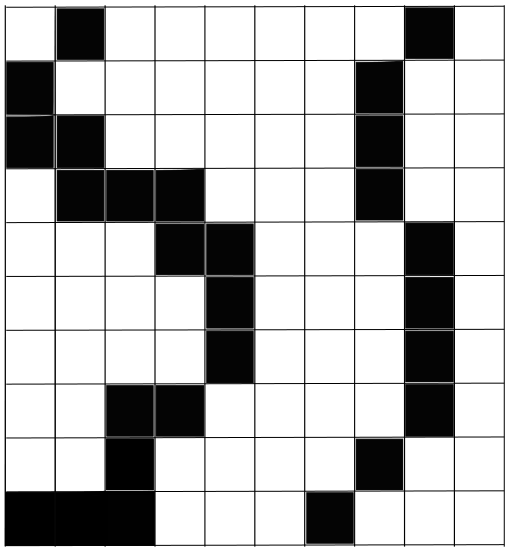
\includegraphics[width=0.5\linewidth]{images/Meander.png}
\end{center}
\end{minipage}
\caption[Two channels with different meander values]{\label{figure:2DMeanderVisualization} Two channels with different meander values. On the left, a bending channel, whose meander value is $\dfrac{2\sqrt{dX^2 + dY^2} + 7dX + 7dY}{\sqrt{82}} \approx 1.86$ when $dX = dY = 1$. The channel on the right's meander value is $\dfrac{4\sqrt{dX^2 + dY^2} + 5dY}{\sqrt{85}}\approx 1.16$ when $dX = dY = 1$ }
\end{figure*}

\begin{algorithm}[t]
\begin{algorithmic}
  \FOR{$\textbf{p} = 0 \to numPixels$}
    \STATE $paths = compilePaths( \textbf{p}, \textsc{MeanderWindow} )$
    \STATE $sum \gets 0$
    \FOR{$ textbf{i} \in paths$}
      \STATE $sum \gets sum + calculateMeander( i )$
    \ENDFOR
    \STATE $setMeander( \textbf{p}, sum / paths.size )$
  \ENDFOR
\end{algorithmic}
\caption[Algorithm to compute the meander field]{\label{algorithm:PixelMeanderValues}The algorithm to compute the meander field. For each pixel $\textbf{p}$, find all paths of size $2 * \textsc{MeanderWindow} + 1$ with $\textbf{p}$ in the center. Then, average each path's meander value according to equation \ref{equation:MeanderCalculation}, and assign this value to $\textbf{p}$.}
\end{algorithm}

\begin{figure*}[t]
\centering
% \begin{tabular}{c|c}
\begin{minipage}[b]{0.75\linewidth}
\begin{center}
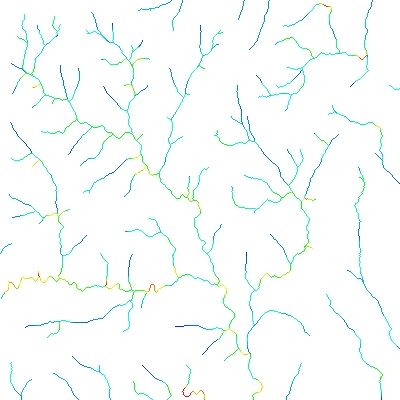
\includegraphics[width=\linewidth]{images/MeanderField_Window15_WithoutWeights.jpg}
\end{center}
\end{minipage}
% &
% \begin{minipage}[b]{0.45\linewidth}
% \begin{center}
% 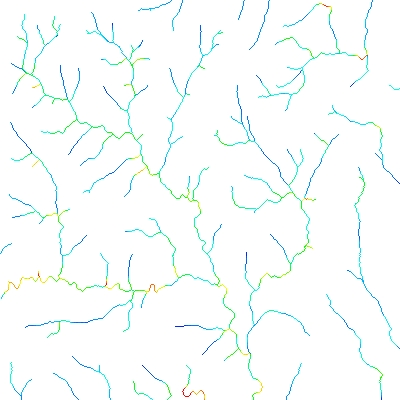
\includegraphics[width=\linewidth]{images/MeanderField_Window15_WithWeights.jpg}
% \end{center}
% \end{minipage} 
% \end{tabular}
\caption[The meander field of MTN2 with a \textsc{MeanderWindow} of 15 pixels]{\label{figure:MeanderFieldVis}The meander field of MTN2 with a \textsc{MeanderWindow} of 15 pixels. Pixels with high meander values (around sharp bends, for instance) are red, while pixels on straightaways are blue.}
% The image to the left was produced without flow weighting. The image to the right was produced with flow weighting.
% \fbox{highlight differences}}
\end{figure*}

\emph{Channel meander} is an important characteristic to the shape and behavior of a channel. It is a measurement of how much the channel bends. Over the course of its lifetime, a channel's bend can sway significantly one way or another, due mainly to erosion of the riverbeds, changing the local meander of the channel. 
A channel's meander is important because it determines 
characteristics of the channel like its velocity and flow pattern.

Like all of the fingerprint characteristics, meander is a pixel-based measurement, and thus results in a meander field. When attempting to quantify how much a segment meanders, there are two main challenges. The first is that the measurement should be continuous as one travels along a channel network. This suggests not assigning a single value for each segment individually, and instead assigning a value for each pixel. At the pixel level, the meander value can change over the course of a channel segment, allowing for smoother transitions between segments. This presents a second problem, however. How should the meander values be calculated at the J points? When a channel with very high meander joins with a channel with low meander, then the junction point (and subsequent joined channel segment) should reflect some sort of average of the two channels. This also helps maintain the continuity goal of the measurement.

Before defining a meander value for each pixel individually, a measurement of meander for a segment is necessary. The meander $m(\textbf{S})$ of a channel segment is defined as the ratio between the total distance traveled by water along the channel to the 2-dimensional euclidean distance between the first pixel ($\textbf{startP}$) and last pixel ($\textbf{endP}$) in the segment:

\begin{align}
\label{equation:MeanderCalculation}
  m(\textbf{S}) = \displaystyle\frac{ ( numDX * dX ) + ( numDY * dY ) + ( numDiag * diagDist) }{ dist( \textbf{startP}, \textbf{endP} ) }
\end{align}

\noindent where $dX$ and $dY$ are the x- and y- grid spacing of the terrain, $numDX$, $numDY$, and $numDiag$ are the number of horizontal, vertical, and diagonal jumps that water takes when following the channel from $\textbf{startP}$ to $\textbf{endP}$, respectively, and $diagDist = \sqrt{dX^{2} + dY^{2}}$. Finally, $dist(\textbf{startP}, \textbf{endP})$ is the 2-norm Euclidean distance measurement between $\textbf{startP}$ and $\textbf{endP}$.

One important property of this measurement is that a perfectly straight segment (whether it be horizontally, vertically, or diagonally straight) will have a meander value of exactly 1.0, a desirable property. This baseline means that the closer a segment's meander value is to 1.0, the straighter it is, regardless of its size or distance from start to finish on the terrain. An example of two meander calculations is found in figure \ref{figure:2DMeanderVisualization}.

% I developed a method for defining what a pixel's meander value means in order to populate the meander field in which every pixel in the channel network is assigned its own. 
The procedure for generating the pixel meander field is found in Algorithm \ref{algorithm:PixelMeanderValues}. The algorithm relies on a user-defined constant parameter known as \textsc{MeanderWindow}, which defines how far up- and down-stream from a pixel $\textbf{p}$ run the paths that are used in the calculation. For each pixel, meander is calculated in three steps:

\begin{enumerate}
  \item Collect all paths that span a distance $\textsc{MeanderWindow}$ from $\textbf{p}$.
  \item For each path, calculate the meander based on equation \ref{equation:MeanderCalculation}.
  \item Compute the average of all paths' meander values, assign it to the pixel's.
\end{enumerate}

All paths will have a maximum length of $2 * \textsc{MeanderWindow} + 1$, but will be shorter for pixels near the start or end of the channel network.
Currently, when calculating a pixel's meander value, it is weighted based on its influence on the total flow entering the pixel.
%  This has, to date, proved to be insignificant to the results. 
A visualization of the pixel meander field of dataset MTN2 with a \textsc{MeanderWindow} size of 15 pixels can be seen in figure \ref{figure:MeanderFieldVis}.

Figure \ref{figure:AverageMeander} is a plot of the average meander value across all pixels in the channel network as it changes with window size. 
% Notice that there is very little difference when flow weights are taken into account, a result consistent with visual observations. 
The average meander value shares a logarithmic relationship with \textsc{MeanderWindow}. This same general behavior holds true for all datasets, though asymptotic to a different bound. 

\begin{figure*}[t]
\centering
% \begin{tabular}{c c}
\begin{minipage}[b]{0.9\linewidth}
\begin{center}
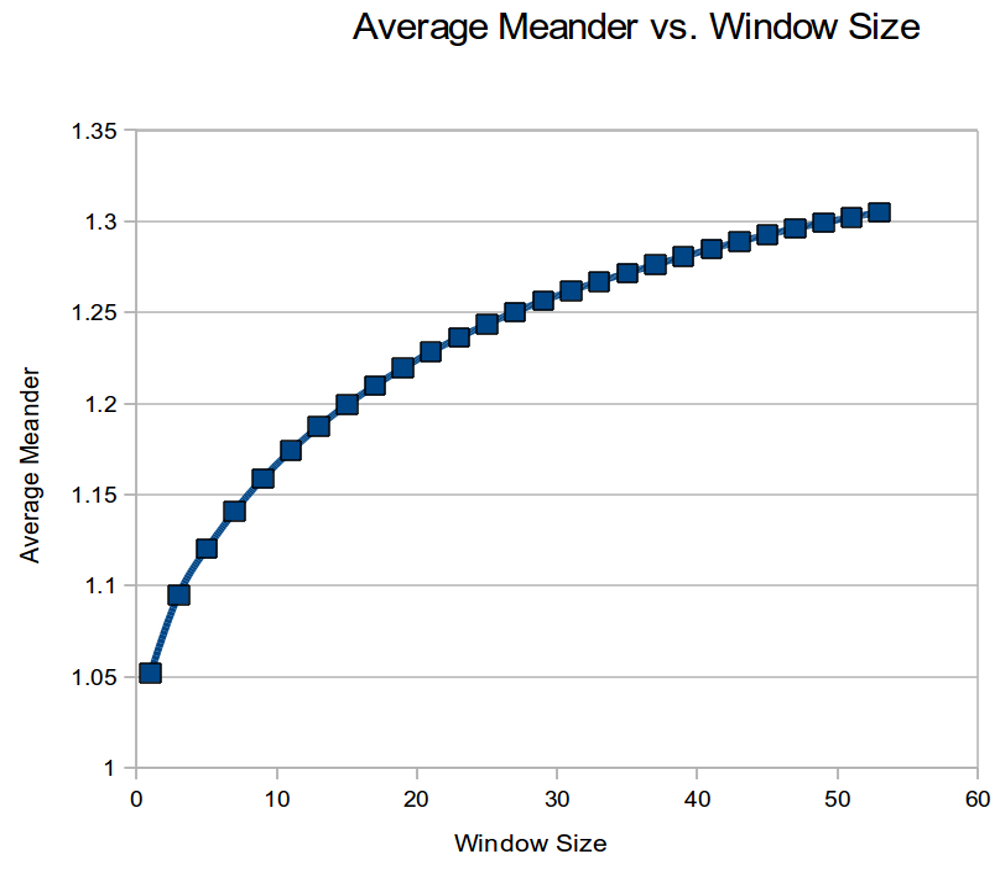
\includegraphics[width=\linewidth]{images/AverageMeander_mtn3_CROPPED.png}
%   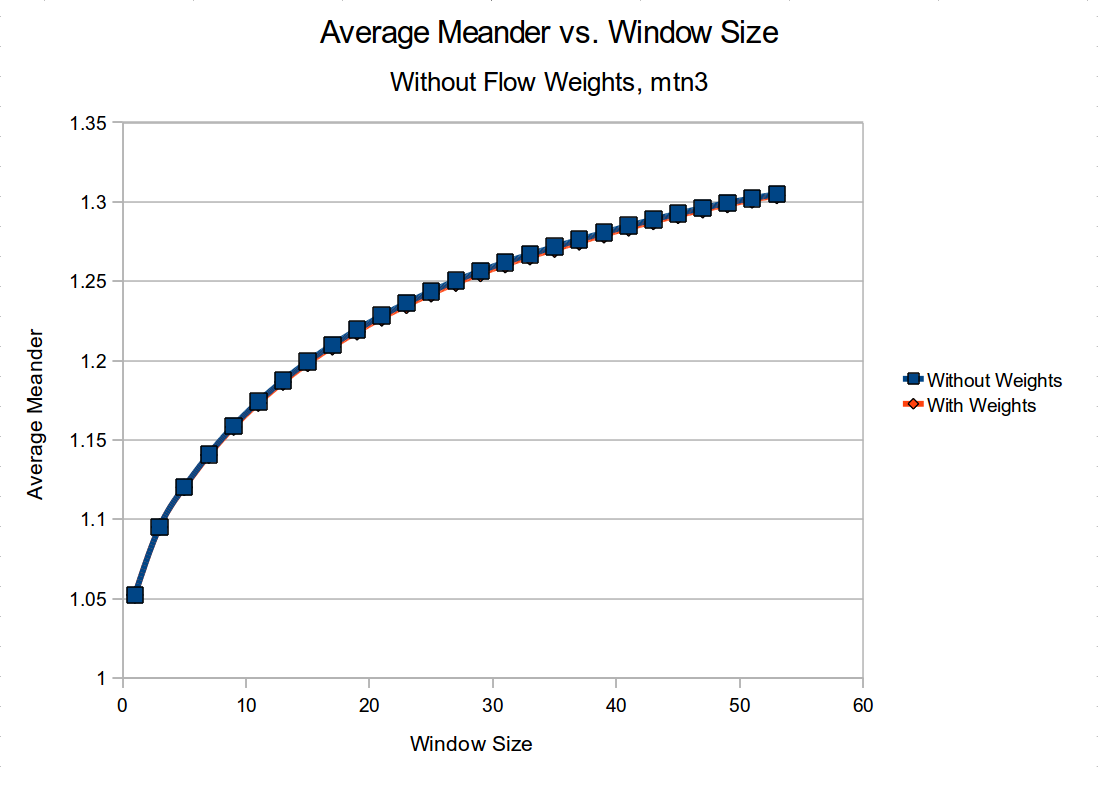
\includegraphics[width=\linewidth]{images/AverageMeanderWithAndWithoutFlowWeights_CROPPED.png}
\end{center}
\end{minipage}
% &
% \begin{minipage}[b]{0.45\linewidth}
% \begin{center}
% 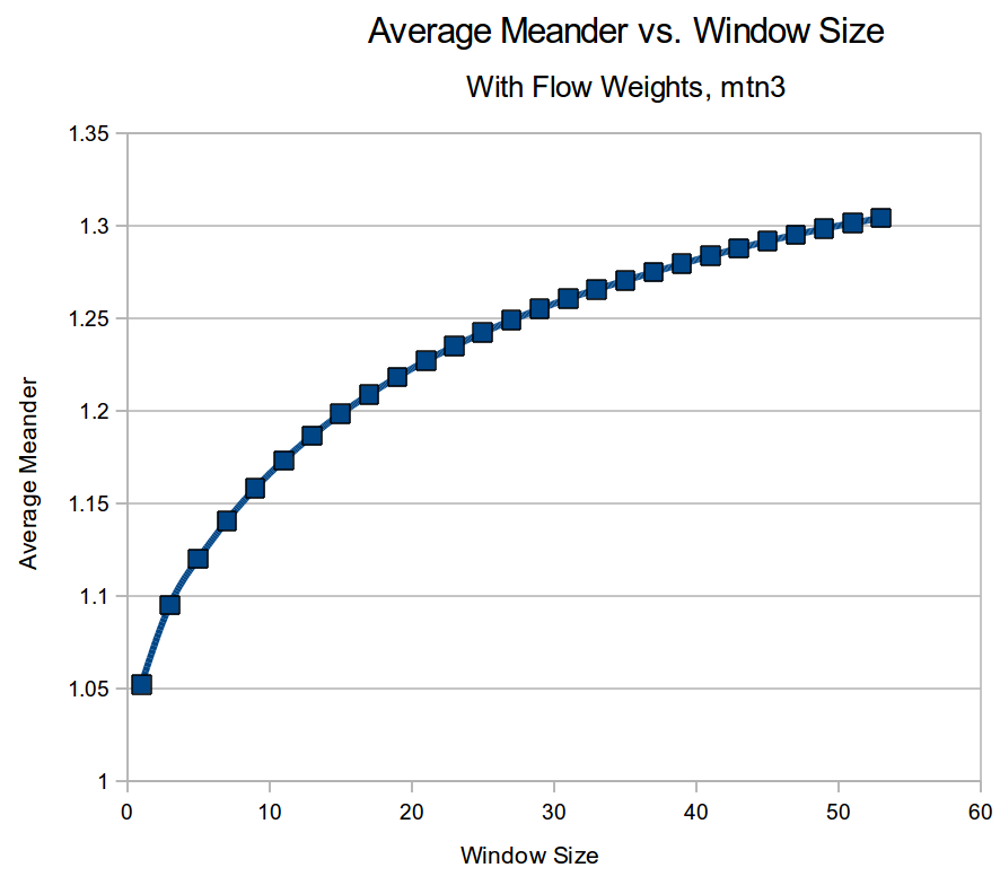
\includegraphics[width=\linewidth]{images/AverageMeander_WithFlowWeights_mtn3_CROPPED.png}
% \end{center}
% \end{minipage} 
% \end{tabular}
\caption[Plot of average meander vs. $\textsc{MeanderWindow}$]{\label{figure:AverageMeander} A plot that demonstrates the behavior of the average meander value across all pixels in the channel network of MTN3 as it changes with \textsc{MeanderWindow}. 
% There is very little difference between the plot without weights (blue points) and the plot with them (red points). 
}
\end{figure*}

In an attempt to normalize meander to a range from 0.0 to 1.0, the maximum possible meander value given \textsc{MeanderWindow} is computed. Intuitively, the channel with the most meander is the channel in which the S and E points are exactly one pixel apart, but the water in the channel travels exactly $2 * \textsc{MeanderWindow} + 1$ diagonal pixels. This maximizes the distance the water travels and minimizes the displacement of the water. However,
% , as can be seen in figure \ref{figure:MaxMeanderPlot}, 
this value grows swiftly. It shares a linear relationship with the window size, as opposed to the logarithmic relationship shared between average meander and window size. After a \textsc{MeanderWindow} of approximately 3 or 4 pixels, the maximum meander value is no longer on the same scale as the average meander value. Since there is not a useful upper bound, the values are not normalized.

Calculation of the maximum possible meander brings up one drawback to the meander measurement. Two wildly varying channel patterns can result in the same meander value. Since the positions of the S and E pixels of a channel are mostly independent of the direction of flow between them, there are many possible channels flowing between them with only diagonal flow directions. 
One possible way to address the problem includes adding discretized way points along the path of a channel, and calculating the Euclidean distance to the end pixel in question, thus increasing the likelihood of finding a different meander value along a channel. These way point values can be weighted and averaged to create a higher resolution meander calculation. This method is equivalent to finding the meander value at a pixel for several \textsc{MeanderWindow} values and weighting and averaging them, creating a more robust calculation.

% \begin{figure*}[t]
% \begin{minipage}[b]{0.9\linewidth}
% \begin{center}
% 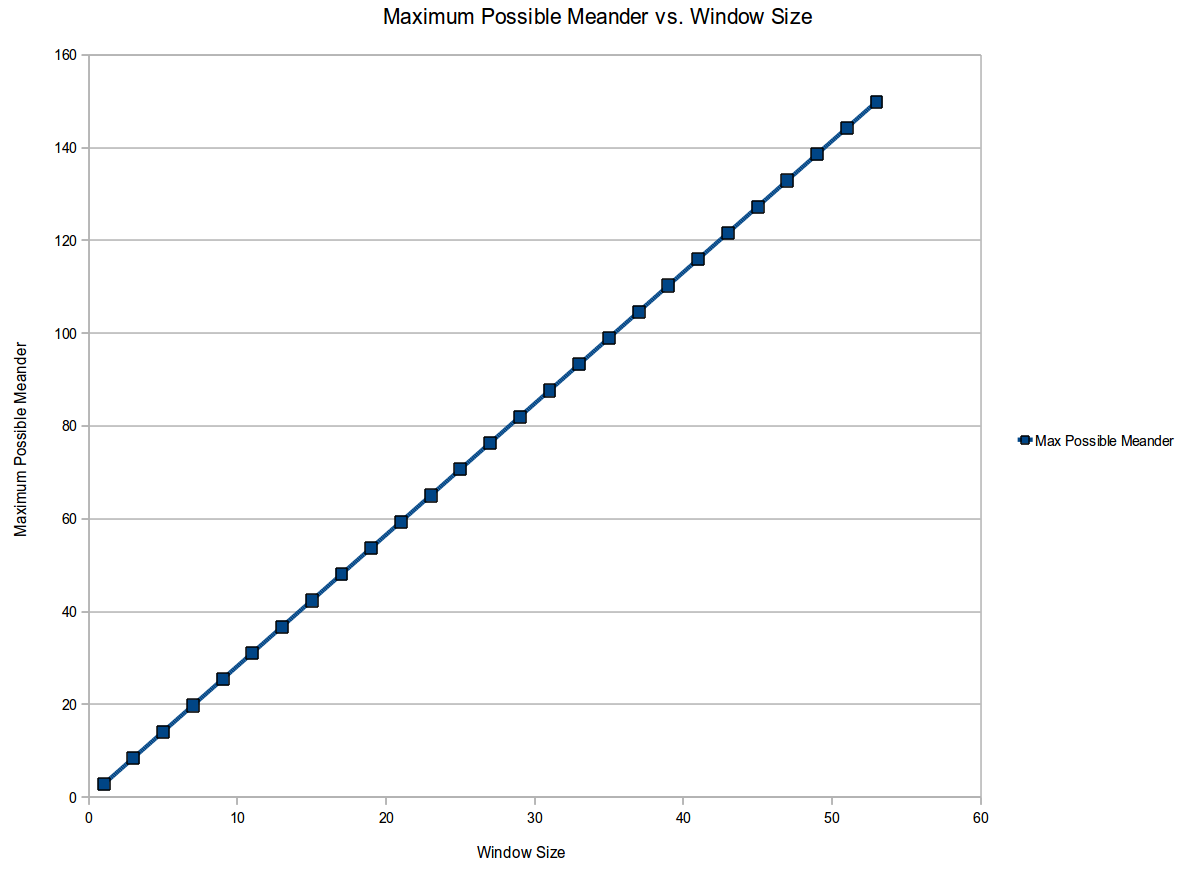
\includegraphics[width=\linewidth]{images/MaximumPossibleMeanderVsWindowSize.png}
% \end{center}
% \end{minipage}
% \caption[Maximum meander value as a function of \textsc{MeanderWindow}]{\label{figure:MaxMeanderPlot} A plot of the maximum meander value as a function of \textsc{MeanderWindow}. Once \textsc{MeanderWindow} passes approximately 3 or 4 pixels, it is no longer comparable to the average meander values presented in \ref{figure:AverageMeander}.}
% \end{figure*}

\subsection{Watersheds and Pixel Load}
\label{section:PixelLoad}

Each channel network on a terrain has its own ``watershed,'' as defined by Band et al. \cite{band86}. 
Watersheds provide a segmentation of the terrain, and allow classification of all pixels (not only those in the channel network itself, as is the case with pixel addresses, discussed in Section \ref{section:PixelIdentification}). 
A pixel whose flow eventually contributes to the flow accumulation of a channel is said to be part of that channel's watershed. A visualization of watershed classification on MTN1 is seen in Figure \ref{figure:WatershedVisualization}. 

The procedure to determine which watershed a pixel is a member of is straightforward, and given in Algorithm \ref{algorithm:WatershedClassification}. 
It consists of walking through each pixel and following its direction of flow until reaching a pixel, \textbf{newPix}, whose watershed has already been identified. Then, the algorithm sets the watershed value of \textbf{p} to that of \textbf{newPix}.
Note that the first digit in the address of any pixel in the addressing scheme presented in Section \ref{section:PixelIdentification} is an identifier for its watershed.

\begin{figure*}[t]
\begin{minipage}[b]{0.9\linewidth}
\centering
% \begin{center}
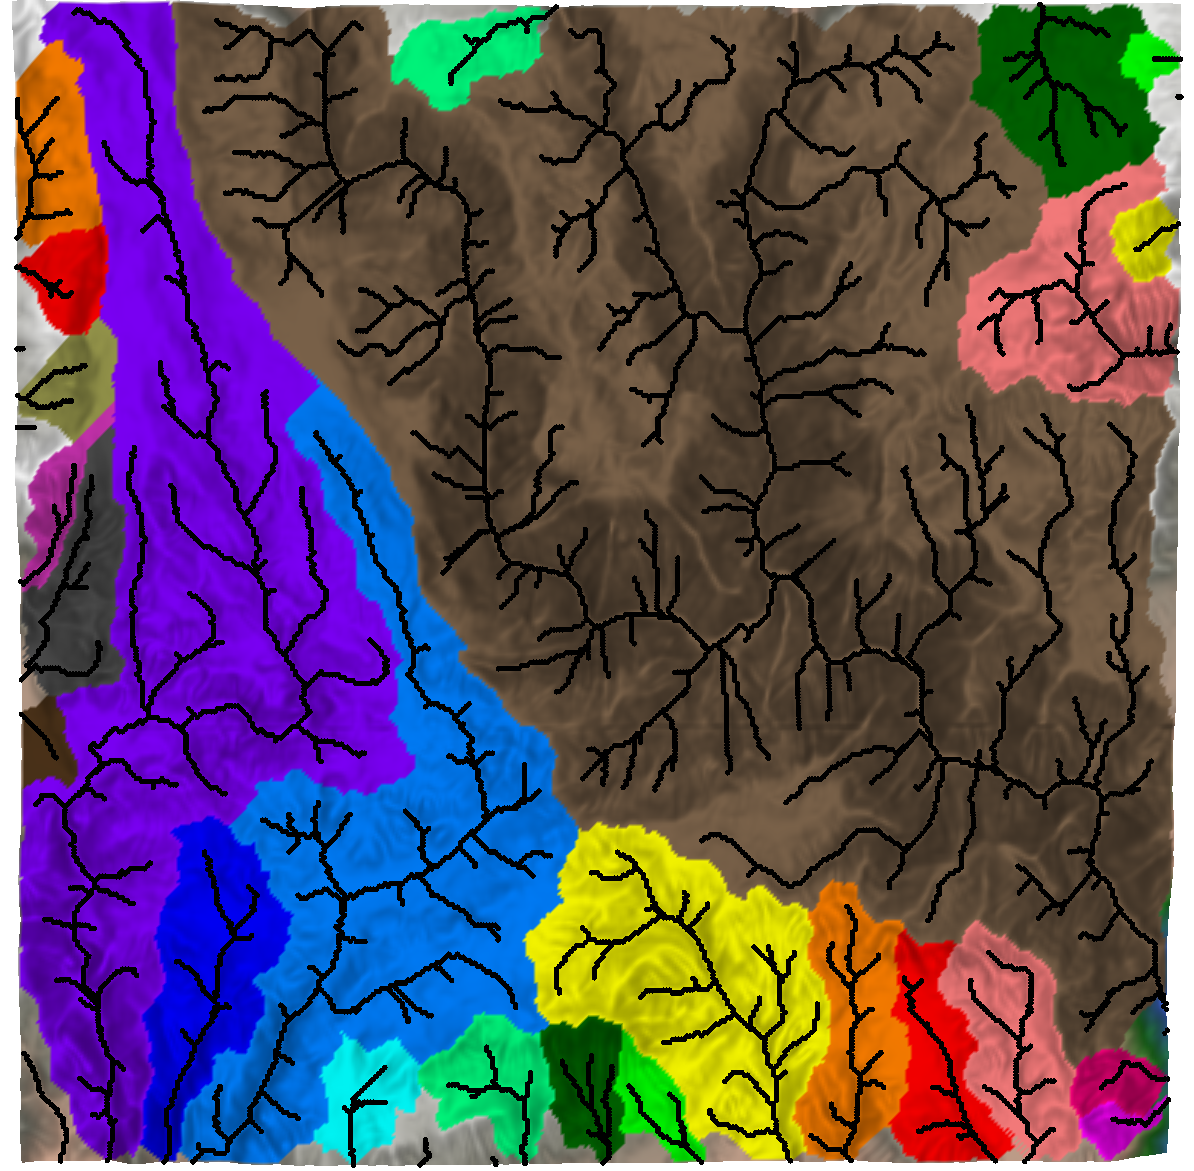
\includegraphics[width=\linewidth]{images/Watersheds_mtn1.png}
% \end{center}
\end{minipage}
\caption[Visualization of watersheds on MTN1]{\label{figure:WatershedVisualization}A visualization of watersheds on MTN1. Each watershed is randomly assigned a color. The brown watershed is the most prolific on MTN1.}
\end{figure*}

\begin{algorithm}[t]
\begin{algorithmic}
  \FOR{$\textbf{p} = 0 \to numPixels$}
    \STATE $newPix \gets \textbf{p}$
    \WHILE{$ isEmpty( getWatershed( \textbf{newPix} ) ) $}
      \STATE $newPix \gets getNextPix( \textbf{newPix} )$
    \ENDWHILE
    \STATE $setWatershed( \textbf{p}, getWatershed( \textbf{newPix} )$
  \ENDFOR
\end{algorithmic}
\caption[The algorithm for assigning a watershed to a pixel]{\label{algorithm:WatershedClassification}The algorithm for assigning a watershed to a pixel. The procedure involves following the direction of flow from a pixel until finding a pixel\textbf{p} whose watershed has already been assigned, and then applying that watershed to \textbf{p}. }
\end{algorithm}

\begin{figure*}[t]
\begin{minipage}[b]{0.9\linewidth}
\begin{center}
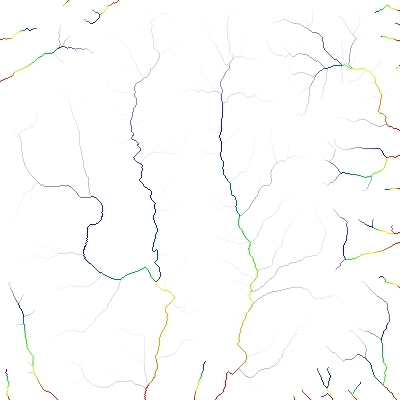
\includegraphics[width=\linewidth]{images/PixelImportance.jpg}
\end{center}
\end{minipage}
\caption[A visualization of pixel load on MTN3]{\label{figure:pixelLoadVisualization}A visualization of pixel load on MTN3. A load near 0 is blue, where the maximum load is red. }
\end{figure*}


It is important to have an indication of how important a pixel is within its watershed. To that end, the \emph{pixel load} of a pixel \textbf{p} is defined to be the ratio of the flow accumulation value of \textbf{p} to the flow accumulation value of \textbf{endP}, where \textbf{endP} is \textbf{p}'s watershed's E pixel. This ratio is shown in Equation \ref{equation:PixelLoad}.

\begin{align}
\label{equation:PixelLoad}
  pixelLoad \left( \textbf{p} \right) = \displaystyle\frac{ flowAccum\left( \textbf{p} \right) }{ flowAccum( \textbf{endP} ) }
\end{align}

Since every channel network has only one E pixel, so too does every watershed. A visualization of the pixel load field, in which every pixel is assigned a value for pixel load, can be seen in figure \ref{figure:pixelLoadVisualization}. The behavior of pixel load makes intuitive sense, as the highest loads will be closer to the E pixels of the watershed. These pixels are deemed to have more ``importance'' to the overall behavior of the watershed than those found near the beginning of tributaries and channel branches.

Pixel load is normalized between the values of 0.0 and 1.0, where the E pixel of each watershed is assigned a value of 1.0. This statistic is calculated independently for each watershed, and thus there is no global information taken into account. 
% In the future, it might be possible to 
It is possible to use pixel load as a thresholded value in place of flow accumulation. For instance, find the channel network using a very low flow threshold, resulting in a very dense network, and then calculate and threshold pixel flow to incrementally adjust the network. 
This weeds out less ``important'' pixels without sacrificing watershed information. 
For some dam siting or path planning algorithms that look locally at the watershed data, this may be more desirable than incrementally thresholding the flow accumulation matrix to determine the channel network.
% , as it does not remove any watersheds and instead narrows the focus to the pixels with highest flood values per watershed.
This process refocuses the extracted pixels to those nearest the E pixels of their respective watersheds. 

Each pixel's load value can also act as a weighting scheme for determining which pixels should be included in the channel network extraction. This is an application of the problem expressed in Section \ref{section:ChoosingAFlowThreshold}.

\subsection{Junction Point Balance}
\label{section:JunctionBalance}

% \fbox{Visualization of JPB with threshold of 0?}

Along the same lines, it is prudent for some applications to either prune or dissect the channel network. An example of this was discussed in Section \ref{section:TerrainCompression}. Pruning is necessary to generalize a channel network, representing it with fewer individual channels while maintaining the overall behavior of the network (Stanislawski and Savino \cite{stanislawski-pruning}, Stanislawski \cite{citeulike:5493394}). Toward this end, a statistic called \emph{junction point balance}, which assigns a value to every J pixel in the channel network based on how balanced its flow value is in terms of the channels that flow into it, has been developed. For each pixel, flow balance is computed according to equation \ref{equation:JBalance}.

\begin{align}
\label{equation:JBalance}
  JBalance( \textbf{ p } ) = \displaystyle\frac{min( flowAccum( nbrs( \textbf{p} ) ) ) }{ max( flowAccum( nbrs( \textbf{p} ) ) ) }
\end{align}

\noindent where $nbrs(\textbf{p})$ is a list of the upstream neighbors of pixel \textbf{p} that are in the channel network, and $min$ and $max$ are as they sound. Junction balance is the reciprocal of the ratio of the maximum to the minimum of the flow accumulation values of the pixels that flow into it. If two channels flow into a J pixel \textbf{p} and contribute the same amount of flow, then \textbf{p} is said to be balanced, and its junction balance value is 1.0. A J point whose contributing segments are very unbalanced will have a very low value of junction balance (nearer 0.0 means more unbalanced). 
% This numbering is slightly counter-intuitive, but it provides for an unbounded balance value for scaling purposes, as very unbalanced J pixels are not limited to a range. 
A visualization of junction balance on MTN3 can be seen in figure \ref{figure:JunctionBalance}.

\begin{figure*}
\begin{minipage}[b]{0.9\linewidth}
\begin{center}
% 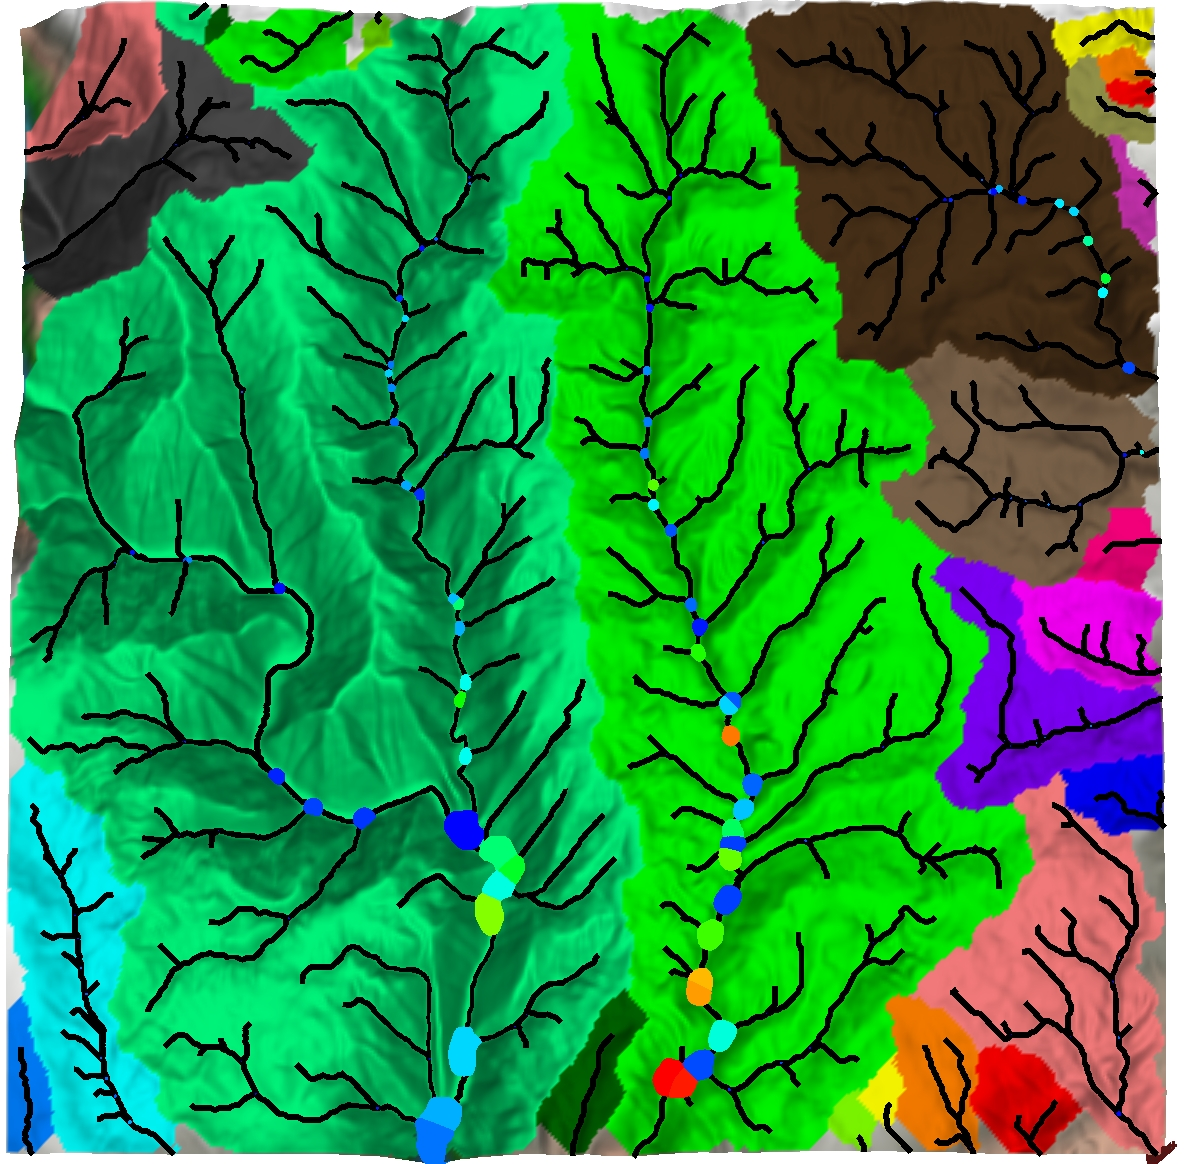
\includegraphics[width=\linewidth]{images/JunctionBalance_mtn3.jpg}
  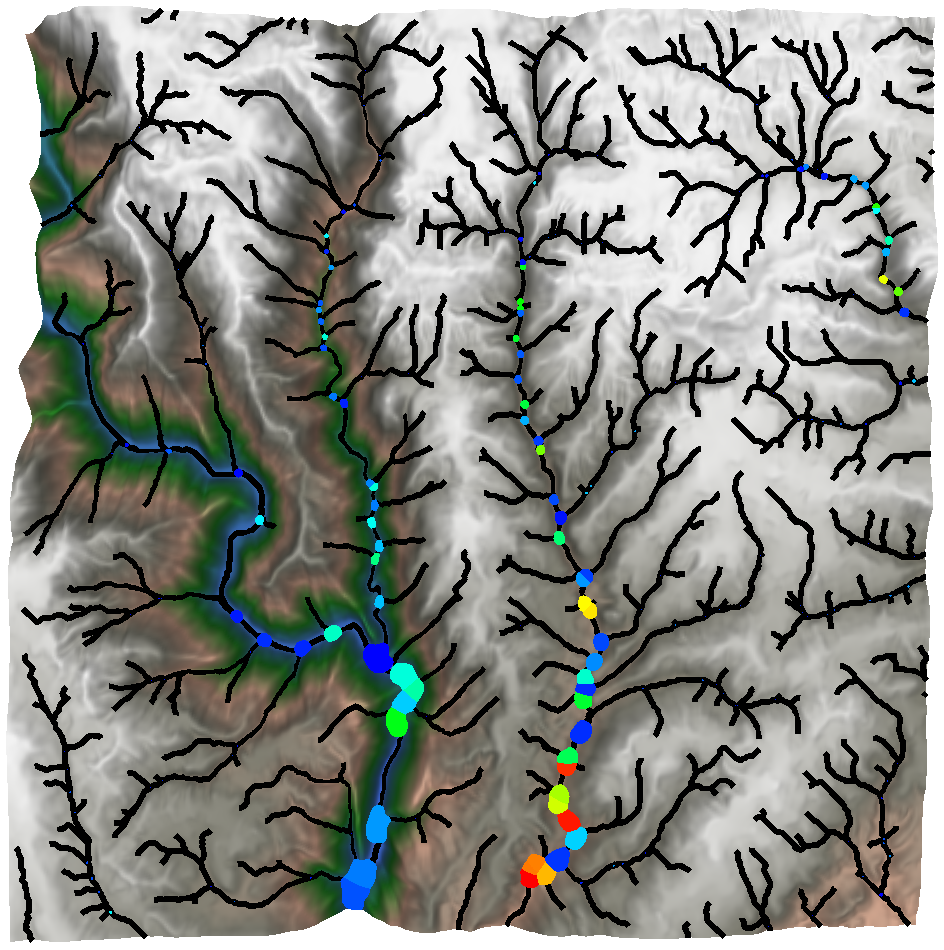
\includegraphics[width=\linewidth]{images/JunctionPointBalanceVisualization_SansWatersheds_cropped.png}
\end{center}
\end{minipage}
\caption[A visualization of junction balance on MTN3]{\label{figure:JunctionBalance}A visualization of junction balance on MTN3. Each junction pixel is assigned a value, and these values are represented by spheres drawn on the terrain. The size of the sphere indicates the total flow accumulation of the J pixel. The color represents the junction balance value, with blue meaning very balanced (near 1.0) and red meaning very unbalanced (very low).
%  Watersheds are drawn for reference. 
}
\end{figure*}

% 
% \begin{figure}
%   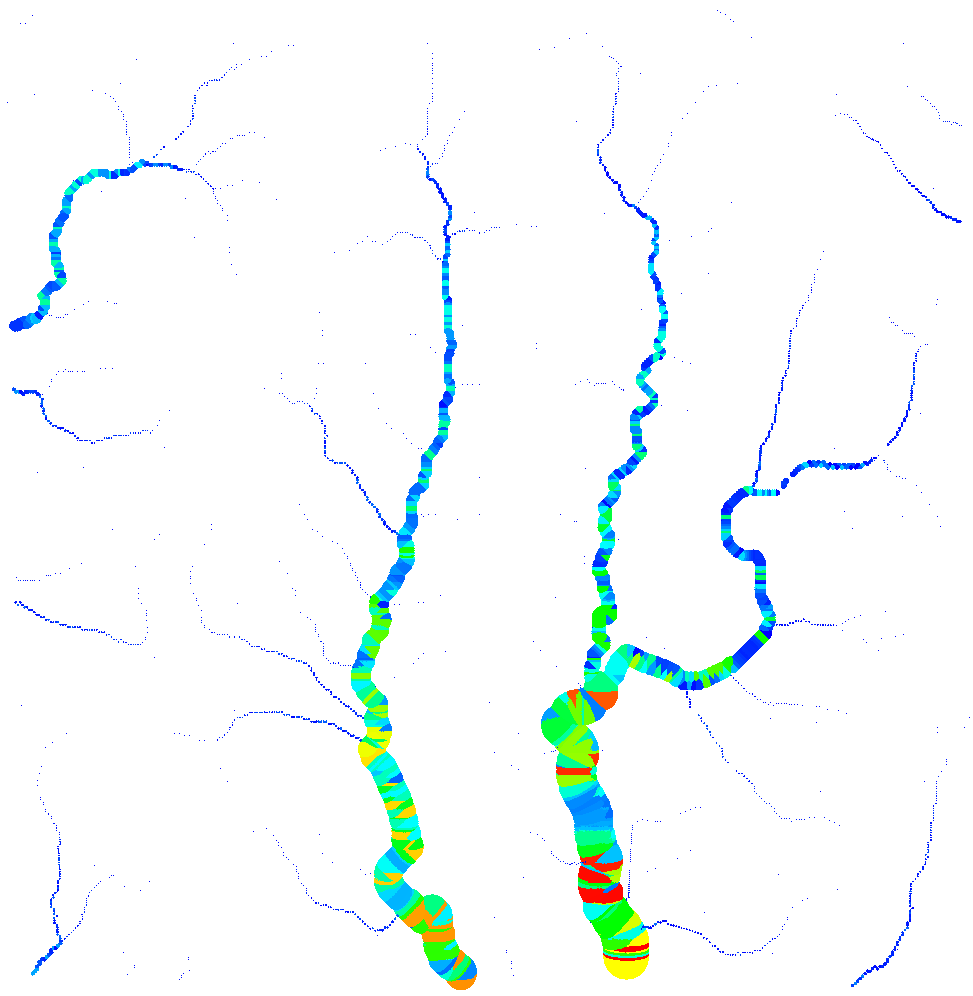
\includegraphics[width=0.9\textwidth]{images/JunctionPoint_AllPixels.png}
%   \caption[Junction Balance for all pixels on MTN3]{\label{figure:JunctionBalanceForAllPixels}This is an image of Junction Balance visualized for all pixels along the terrain.}
% \end{figure}


\begin{figure*}[t]
\begin{minipage}[b]{0.9\linewidth}
\begin{center}
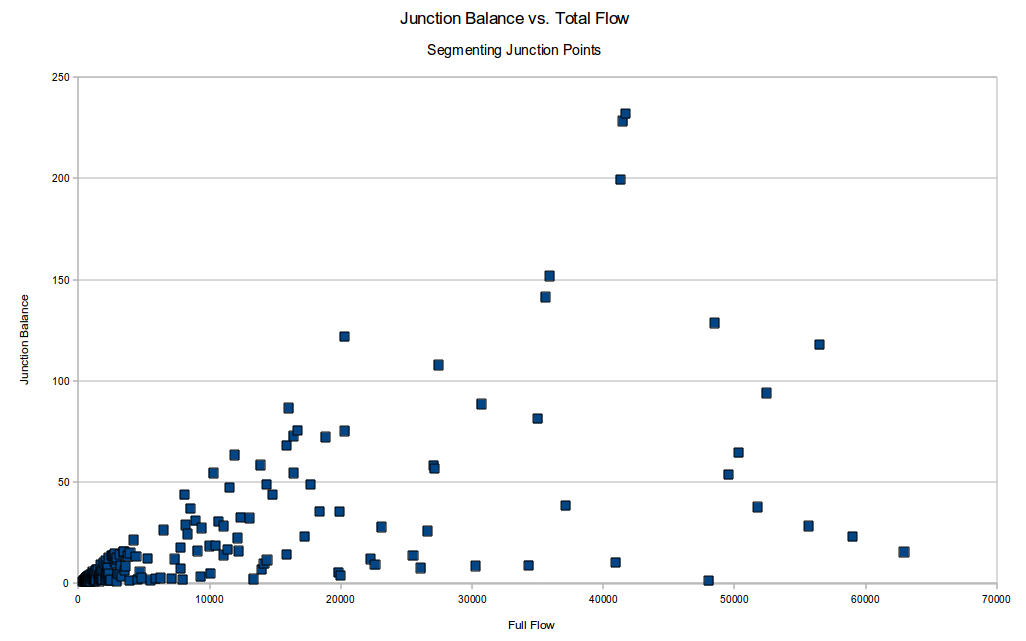
\includegraphics[width=\linewidth]{images/JunctionBalanceVsFullFlow.png}
\end{center}
\end{minipage}
\caption[A plot of junction balance vs. flow accumulation]{\label{figure:BalanceVsFlow}A plot of junction balance vs. flow accumulation. No junction points exist in the upper left quadrant of the graph, which is intuitive because there is a limit to how unbalanced a pixel early in a channel network can be.}
\end{figure*}
% 



\begin{figure}
\centering
\begin{minipage}{0.55\linewidth}
\begin{minipage}{\textwidth}
\begin{center}
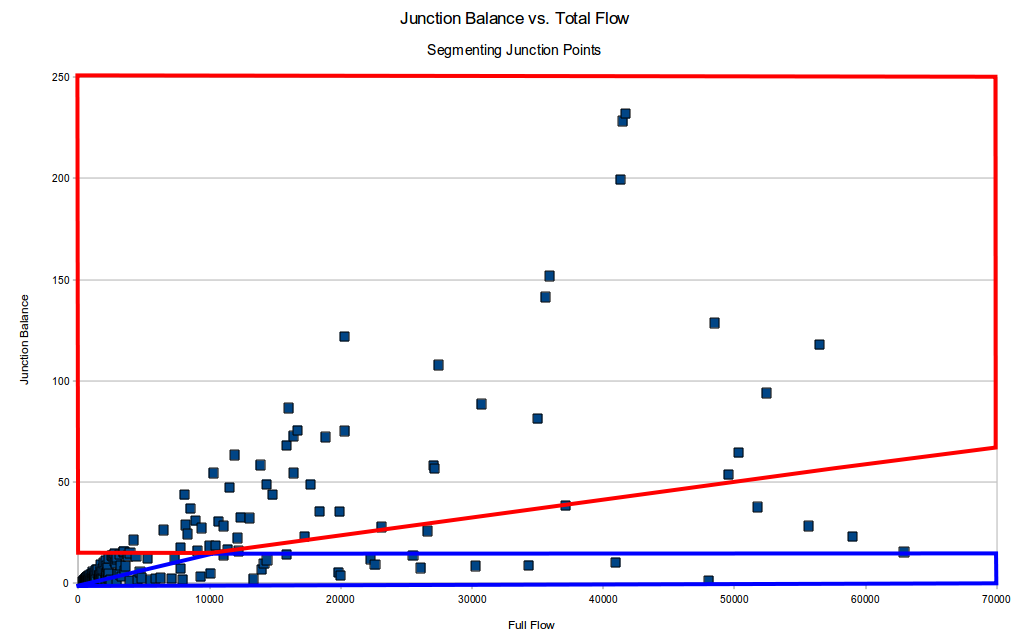
\includegraphics[width=\linewidth]{images/JunctionBalanceVsFullFlow_Annotated_WithRatio_AndBalanceLimit.png}
\end{center}
\end{minipage}
\\
\begin{minipage}{0.99\textwidth}
\begin{center}
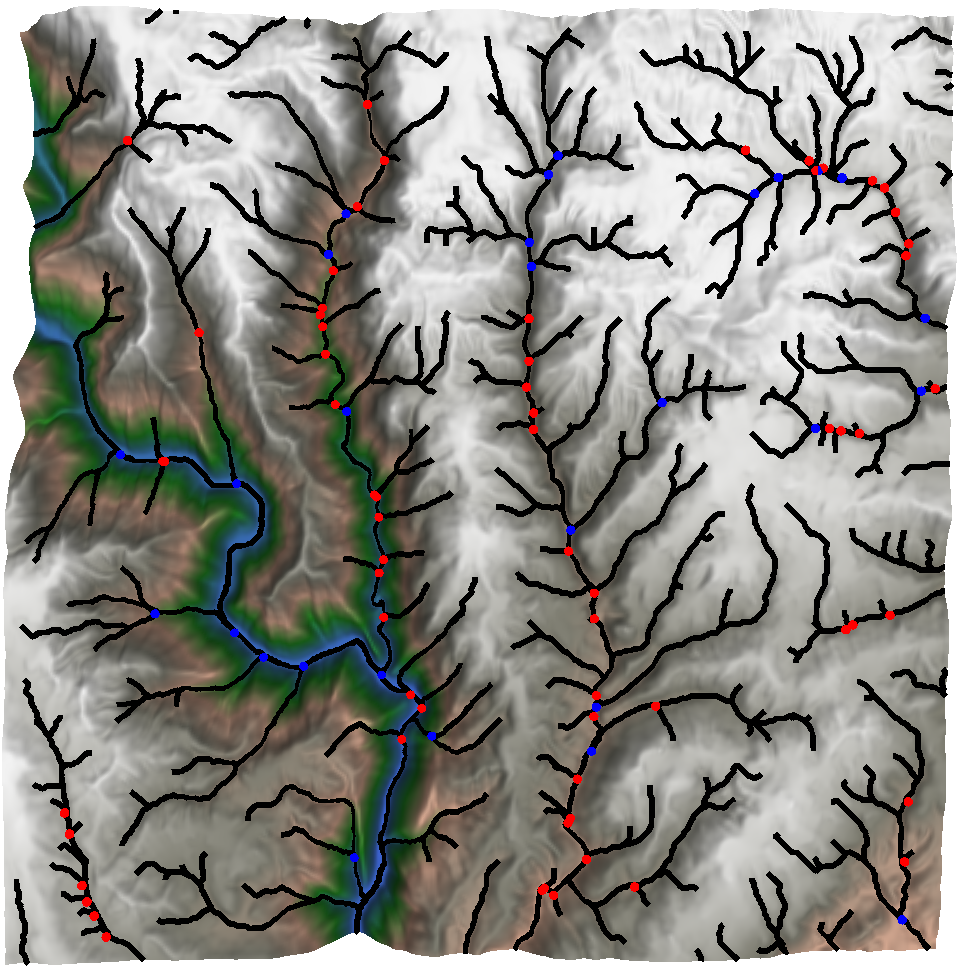
\includegraphics[width=\linewidth]{images/FlowToBalanceRatioWithBalanceLimitOf10.png}
\end{center}
\end{minipage}
\end{minipage}
\caption[A segmentation for pruning and dissecting]{\label{figure:SegmentedJunctionBalance2} Top: Segmentation of the junction pixels into two categories, those above the balance threshold and with flow/balance ratios less than 1000.0 in red, and vice versa in blue. Bottom: The candidate junction pixels circled in red and blue in the graph are marked with corresponding dots on MTN3.}
\end{figure}

There are two primary watersheds on MTN3, dark green (to the left) and light green (in the middle). The junction points in the left watershed are all fairly balanced, meaning that they are mostly in the blue to green range. This indicates a lack of small, insignificant tributaries joining major channels. The right watershed, however, has many junction points that are in the yellow to red range, indicating the existence of small, insignificant tributaries. This is especially true near the bottom of the watershed, when the primary channel's flow has grown significantly, and so small tributaries are going to provide for very unbalanced junction points.


% Looking at the junction balance for all pixels on MTN3, as seen in Figure \ref{figure:JunctionBalanceForAllPixels}, it is immediately clear that the majority of junction points on the network are pixels within the channel network. This makes intuitive sense, since those are the pixels with the largest flow accumulations. Also to be expected is the fact that the right watershed has many more red junction points than the 


%JUNCTION BALANCE HISTOGRAM WILL GO HERE

Junction balance can be used to identify junction points that can be pruned (the smaller of the joining channels being removed from the channel network) or dissected (each of the joining channels separated to become its own channel network). 
% As an example, let us identify J pixels on MTN3 that we would like to dissect, as seen in Figure \ref{figure:DissectionPixelGoal}). 
% 
% \begin{figure*}[t]
% \begin{minipage}[b]{0.9\linewidth}
% \begin{center}
% 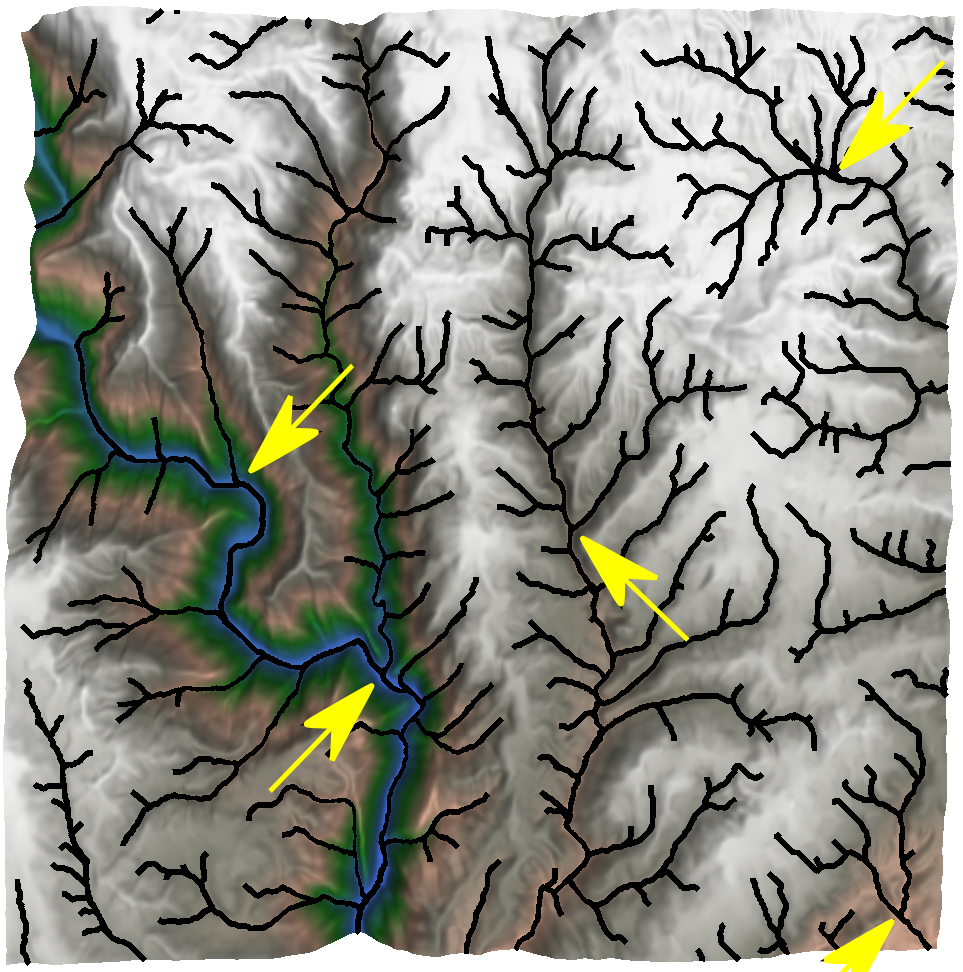
\includegraphics[width=\linewidth]{images/Terrain_mtn3_DissectionPointsGoal.png}
% \end{center}
% \end{minipage}
% \caption[Identification of five possible dissection points]{\label{figure:DissectionPixelGoal}Identification of five junction pixels on MTN3 that represent the joining of two well-balanced channels that could represent ideal dissection points.}
% \end{figure*}
% 
% With these goal pixels in mind, 
The relationship between junction balance and the total flow accumulation values of the various J pixels on the terrain was examined. This data is seen in figure \ref{figure:BalanceVsFlow}. The goal is to identify which pixels should be pruned and which should be dissected. The pixels with very high balance values should be identified as candidates for pruning, as they represent small tributaries joining with much larger channels. Those with very low balance values but high flow values should be identified as candidates for dissection, as they represent the joining of two large and equally sized channel networks. The pixels to ignore, such as those with very low flow accumulation, should also be identified, as they tend to exist in very high elevations toward the beginning of channel networks. 

With these ideas in mind, the junction points were segmented. Two constraints were used to create a point selection scheme. The first is a limit on the total balance considered, and the second is the flow/balance ratio line. The points are then segmented as in \ref{figure:SegmentedJunctionBalance2}, where points with flow/balance ratios of less than 1000.0 and junction balance of greater than 10.0 are marked red, and vice-versa for blue.

The major junction points can be found in the bottom right quadrant (blue bounded area), when the flow is large but the balance is small. These are junction points in which two (or more) major channels converge. When looking for points at which a segmentation can occur (dividing the channel network into two channel networks), these are the points of interest. 
Those data points with high flow and high balance metric score (red encircled area) represent junction points in which small tributaries join major channels. These points are prime candidates for trimming operations, in which smaller tributaries that do not contribute much to the main channel can be pruned off.

% 
Notice the channel network in the bottom left corner, in which all small and (seemingly) inconsequential tributaries are candidates for pruning.
% Also, notice that every pixel that was identified earlier as a potential dissection pixel is selected in this scheme. This scheme identifies all of the dissection pixels in our goal image, figure \ref{figure:DissectionPixelGoal}.
In addition, major junction points are marked for possible sources for dissection. This is a quick method for identifying candidates that a user can then use to make decisions about where and how to dissect and prune the channel network. These can also be weighted by the Pixel Load for a better determination.


\section{Terrain Fingerprints as Distance Metrics}
\label{section:FingerprintsAsMetrics}

% \fbox{ RERUN RESULTS!}

Fingerprints provide statistical descriptors of the terrain surface. Comparing them is a worthwhile challenge, as it provides another measure of dissimilarity between datasets as well as further geometrical insight into the meaning of the statistics. Therefore, a measure of dissimilarity, similar to those presented in Section \ref{section:TerrainDistances}, is necessary. Since fingerprint characteristics can be represented by 2D sparse probability distributions (by simply normalizing the matrix of values), the Earth Mover's Distance (EMD), presented by Rubner et al. \cite{Rubner:2000:EMD:365875.365881} (code based on the method by Lin and Okada \cite{Ling:2007:EEM:1263143.1263456}), provides a useful measure of dissimilarity for them.

In order to utilize EMD, a \emph{ground distance} is necessary. This is a measure of distance between two points in the distributions. The Euclidean distance ($L_{2}$ norm) works sufficiently in this case,
% Euclidean distances do not work in their natural form for the fingerprints because the pixel-space scale (x,y coordinates) and the scale of the pixel values (depends on the characteristic) may be vastly different from one another. 
% Therefore, the pixel's value ($\textbf{p}_z$) is weighted differently for each.
% 
since each of the characteristics is on the same scale (including Meander, which hovers around 1.0 but not in the same $[0.0, 1.0]$ range as Pixel Load and Junction Point Balance).
% , it is possible to soften the impact of the pixel-space coordinates in the Euclidean distance calculation. Therefore, the x- and y-coordinates of the pixels are weighted by a factor of 0.01. Two pixels whose values are on opposite ends of their possible range will incur an Earth Mover's penalty equivalent to moving a distance of 100 on the xy-plane, a hefty cost.


Each statistic is converted into a histogram with $n$ bins. For this work, $n = 500$ has been sufficient. 
Each bin of the histogram counts the number of pixels whose values fall into the corresponding range ($\frac{1}{n}^{th}$ of the total range of the values). 
They are then normalized, because it is recommended that EMD be used to measure the dissimilarity between sets with equal volume (measuring differences in their overall shapes). 


\begin{table}[t]
  \centering
  \caption[Minimum dissimilarity values in tests for different terrain fingerprint characteristics]{\label{table:FingerprintMetrics} This table presents the minimum dissimilarity found for each of the terrain fingerprint characteristics (Meander, Pixel Load, and Junction Point Balance) for each of the six datasets. These numbers do not have a direct geometrical meaning, but do provide a measure of dissimilarity between datasets. The corresponding network densities are given in parentheses.}
  \begin{tabular}{ | c | c | c | c | }
    \hline
      & \textbf{Meander} & \textbf{Pixel Load} & \textbf{Junction Balance} \\
    \hline
    HILL1 & 5.79 (8) & 4.55 (35) & 2.04 (13) \\ 
    HILL2 & 2.82 (15) & 3.63 (32) & 2.44 (23) \\ 
    HILL3 & 6.08 (13) & 2.86 (39) & 2.60 (38) \\
    MTN1 & 1.88 (40) & 1.25 (12) & 1.69 (15) \\
    MTN2 & 0.59 (14) & 0.88 (14) & 1.84 (13) \\
    MTN3 & 1.61 (32) & 0.68 (15) & 1.13 (19) \\
    \hline
  \end{tabular}
%  divided by function family. The top third of the table refers to data for linear drill shapes, the middle third to quadratic drill shapes, and the bottom third to cubic drill shapes. The results for each of the six datasets found in Figure \ref{figure:SixDatasets} is reported.}
\end{table}



EMD is then applied to the normalized histograms.
If the channel networks are sparse, then the 0-bin of the resulting histogram is ignored, and this is another measure of the dissimilarity of two channel networks. However, building a channel network that includes 100\% of the pixels allows for EMD to be used to determine the dissimilarity between the terrains' hydrographic characteristics. For instance, dense Pixel Load differences are really a measure of how different water flow patterns are within corresponding watersheds.

The experiment performed in Section \ref{section:DrillAccuracyTrials} was repeated using the sparse fingerprints' EMD as the metric. It is important to note that EMD is designed as a measure of dissimilarity, and as such is not normalized to the range [0.0, 1.0] as other metrics are. Results of these tests are seen in Table \ref{table:FingerprintMetrics}.

As expected, minimum dissimilarity measures are lower for the MTN datasets. Their smaller values for meander indicate that the shape of the channels on the MTN datasets match much more closely, which makes intuitive sense given the clarity of channel of the MTN terrains. More interestingly, pixel load values are very close for the MTN datasets, indicating that the overall watersheds match as well. Higher meander and pixel load values for the HILL datasets are indicate that small elevation errors do, in fact, result in widely varying channel networks, including both the shapes of the channels and their branching patterns.

Junction balance distances were fairly low, and much closer between the two dataset categorizations. What is interesting is the wide variety of network densities that resulted in the minimum junction point balance distance. Further investigation determined that the overall variation in these distances was very small across all densities. For instance, the next three best fits for HILL1 after a density of 13\% were 4\%, 5\%, and 10\%. Overall, it is difficult to determine a trend for junction point balance's distance data.

This is also the case for the meander data. The standard deviations for the meander data were considerably higher than those of the other two metrics. This was especially true for the HILL datasets, as to be expected, lending further evidence to the difficulty in relying on the extracted channel networks for datasets with low frequency features. 

To rely on this hydrography information as a true dissimilarity metric, it is necessary to combine the three characteristics. Meander values are too varying to use on their own, but when clear channels are seen in the terrain, they are a valuable measure of the shape of the resulting network. Pixel load, when applied to all pixels in a terrain, is a good overall indicator of hydrography behavior, and thus is a good measure of introduced hydrography error when regenerating a terrain. Overall, junction balance is a tight measurement (with low standard deviation) for clearly defined channels. These results point toward a need for a pre-processing step when studying a terrain that determines and categorizes the statistics (both the fingerprint statistics and those for the drill representation, such as drill radius) that will best represent the surface, as discussed in Section \ref{section:DrillSummaryAndFutureWork}.


% \fbox{FILL IN NEW RESULTS}
% Results are largely the same as those reported in Section \ref{section:FamiliesOfFunctions}. In general, dissimilarities measured on the HILL datasets were larger than those in the MTN sets. 
% Once again, this can be somewhat attributed to the fact that small changes in elevations in flat areas of the terrain can cause abrupt and significant alterations in the channel network. Since these flat areas are more common in the HILL datasets, this situation arises more often for them.
% This is also the primary reason that the drill operator represents MTN datasets with less overall error, as the channel networks in the MTN datasets are less fickle with regard to elevation error.
% 
% All measurements were on the same approximate scale a majority of the time. However, for the HILL datasets Pixel Load was often considerably larger than the other measurements. I attribute this once again to a small change in the elevation along relatively flat areas. If a few pixels' flow is added to a different watershed, then the Pixel Load values can be significantly different. Therefore, Pixel Load can be used as a measurement of how closely two watershed clusterings are. In this light, it is not surprising that MTN datasets' regenerations performed better for this characteristic.
% 
% It should also be noted that Linear and Quadratic drill shapes' measurements are not as clear-cut as when using RMSE and SSRMSE, as far as which is the better representation. Some datasets' characteristics are better represented by a linear drill while others are better fit by the quadratic. However, for the MTN datasets, the linear drill shape is still overwhelmingly more accurate when one takes into account the best several fits. For instance, for MTN1, 17 of the top 20 Meander dissimilarity values were linear drill shapes, 13 of the top 20 for Pixel Load, and 15 of the top 20 for Junction Point Balance.
% With the exception of HILL2, the cubic drill shape is still universally the worst of the drills. 



These measurements are very fast to calculate. The slowest portion of the process is the extraction of the channel network (discussed in Section \ref{section:ChannelNetworkExtraction}, and is $O\left(n \log n\right)$). Meander calculation takes
$O\left( m \textsc{MeanderWindow} \right) $ time once this has been completed, where $m$ is the number of pixels in the extracted channel network. Pixel Load and Junction Point Balance are computed in $O\left(m\right)$ time. Essentially, each statistic requires a single pass through the channel network and a single (or $\textsc{MeanderWindow}$) calculation(s) per pixel.

\section{Summary and Future Work of Terrain Fingerprints}

This section presented the terrain fingerprint, a series of statistics drawn from the channel network extracted from a terrain. A fingerprint is determined by first calculating the flow accumulation and flow direction fields of a terrain, then thresholding the flow accumulation matrix to determine which pixels are part of the channel network. This threshold is determined by a weighted algorithm whose weighting is based on the position of the pixel's elevation from the maximum elevation, as well as its index in the pixels when ordered by elevation. Once this series of connected pixels is extracted, the individual pixels are identified as: the start (S), end (E), middle (C), or junction points (J) of the channels. Pixels are assigned addresses, and from the flow direction and flow accumulation fields, terrain characteristics, such as pixel meander, pixel load, and junction point balance, are calculated.

These statistics provide a variety of uses. The first is as a sparse representation of the hydrography of the terrain that statistically encodes the behavior of water on the surface in a compact and descriptive manner. This sparse representation can then be used as a measure of dissimilarity between two datasets, using the Earth Mover's Distance metric for probability distributions by building histograms from the sparse characteristics. 
% Extracting the statistics from denser channel networks provides more information about the terrain as a whole, such as the behavior of water within each watershed.
This provides a measure of how alike or not the extracted channel networks of two terrains are, and ultimately is more useful on mountainous terrains with more clearly defined network shapes. However, with the help of a pre-processing step, this could become a powerful tool for categorizing and properly analyzing terrain surfaces for use when representing the terrain with a series of drill operations.

In addition, the statistics themselves are useful for various applications. Pixel load provides a natural weighting scheme for pixels in the extracted channel network, and junction balance provides data for pruning and dissection processes. If applied to the same terrain over multiple years, the pixel meander provides a statistical measure of the behavior of the bends of channels on the surface.

% These are the first of many possible statistical descriptors of terrain surfaces. Describing the surface of the terrain with more complex probability distributions, as described in Section \ref{section:ShapeAnalysisTechniques}, would provide means for shape matching techniques to apply to terrains. With advancing computer vision techniques, given a small piece of data, one might be able to quickly scan large geographical databases to find matching sections, determining the location of said data. 

Each of the characteristics for terrain fingerprints will be explored further.
%  as future work. 
% This thesis has only touched on the surface of the implications of representing and comparing terrains based on the Meander, Pixel Load, and Junction Point Balance distributions. 
Pixel Load will be used as a weighting scheme for work in the future, and Junction Point Balance will be used to prune off uninteresting or unimportant channels. Meander will be used in a dense field to predict the behavior of the channel network over time. All three characteristics will be used to develop a representation of the terrain and compress it. 


